\documentclass[UTF8, 11pt, oneside]{ctexart}

\usepackage{float}

\usepackage{geometry}
\geometry{a4paper,left=2cm,right=2cm,top=2cm,bottom=1cm}

\usepackage{graphicx}

\usepackage{hyperref}
\hypersetup{colorlinks=true, linkcolor=red}

\linespread{1.6}


\def\articletitle{出售铀矿的收入要上交俄罗斯5成,尼日尔对此感恩戴德}

\usepackage{fancyhdr}
\usepackage{ifthen}
\pagestyle{fancy}
\fancyhf{}
\setlength{\headheight}{14pt}
\fancyhead[R]{\ifthenelse{\value{page}>1}{\thepage}{}}
\fancyhead[C]{\ifthenelse{\value{page}>1}{\articletitle}{}}
\renewcommand\headrulewidth{0pt}

\usepackage{tcolorbox}
\tcbuselibrary{skins}


\newcommand{\zd}[1]{\textbf{\textcolor[RGB]{123,12,0}{#1}}} % 重点

\newcommand{\yh}[1]{% 引用
    \begin{tcolorbox}[enhanced,
        frame hidden, interior hidden,
        before skip = 5mm, left skip=10mm,
        borderline west={5pt}{0pt}{gray!50}]
        #1
    \end{tcolorbox}
}

\newcommand{\biaoti}[1]{% 标题
    \section*{#1}
}

\begin{document}

\begin{center}
    \LARGE{\articletitle\footnotemark}
\end{center}
\footnotetext{
    原文出自公众号“远方青木”的文章 《\href{https://mp.weixin.qq.com/s/OhBFX73Sw0se_NxOno5cyA}{\articletitle}》
}

这次巴黎奥运会法国特别针对俄罗斯,以俄乌战争的名义禁止俄罗斯参加奥运会。

但法国没禁以色列,而其他欧洲国家如德国等也没那么反对俄罗斯,这说明法国和俄罗斯还有其他恩怨。

\zd{事实确实如此,俄罗斯最近在非洲把法国搞的够呛。}

尼日尔,世界第七大铀矿生产国,全国70\%的外贸出口金额来自于出售铀矿,整个欧盟采购的铀矿1/4来自于尼日尔,该国长期受到法国控制。

2023年7月26日,尼日尔总统卫队发动政变,扣押了亲法总统巴祖姆,随后推翻了巴祖姆政权,组建了一个亲俄政权。

虽然俄罗斯官方没有承认,但在政变成功后尼日尔的民众上街兴奋的高呼“瓦格纳”的名号,而瓦格纳正是俄罗斯麾下的雇佣兵军团。

\begin{figure}[H]
    \centering
    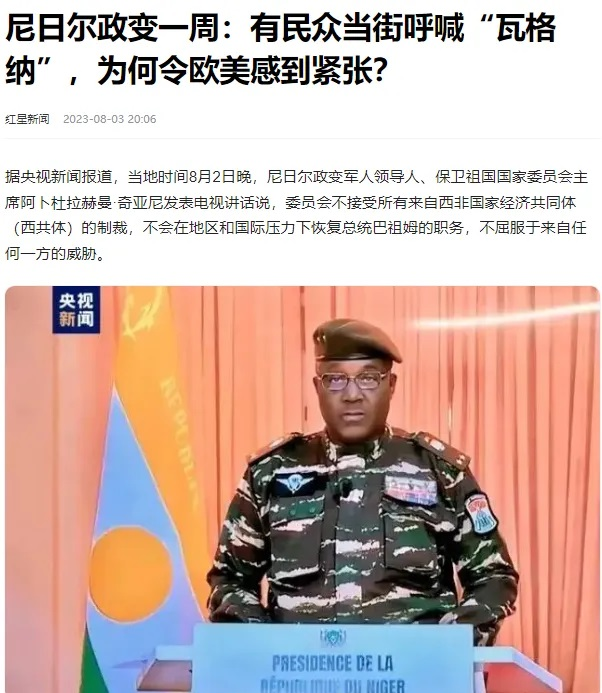
\includegraphics[width=9cm]{2024-08-08-001.jpg}
\end{figure}

对于新生的尼日尔政权,俄罗斯承诺提供保护,瓦格纳的部队直接驻扎在了尼日尔,而这个“保护费”的代价是以后尼日尔出售铀矿的收入要交给俄罗斯5成。

\zd{全国唯一经济支柱以后要凭空分5成出去,对于这一条件,尼日尔感恩戴德。}

因为在被俄罗斯的瓦格纳“解放”之前,尼日尔所有出售铀矿的收入,要上交给法国92\%。

因为负责开采尼日尔铀矿的阿海珐公司,其87\%的股权属于法国政府,这个股权分配指的是净利润,需要扣除成本,然后开采过程还需要法国的“科米纳克公司”等参与分润。

七七八八算下来,每年出口铀矿的营收款尼日尔需要给法国92\%,这些分配条款都是白纸黑字写在尼日尔亲笔签下的条约《尼日尔-法国条例》里的。

但剩下的8\%,尼日尔也不能随便花,需要先把这些钱存在法国指定的银行,每一分钱的动用都必须经过法国的审批,且只能购买指定的法国商品。

\zd{有一年因为“汇率波动”外加法国银行结算的“效率低下”,结果尼日尔人辛辛苦苦挖了一年铀矿,最后算账算下来,整个尼日尔倒欠法国1000多万美元。}

如果瓦格纳不来,尼日尔就只能世世代代的和法国按这种条约分配出售铀矿的收入。

但如今瓦格纳来了,把法国赶跑了,那这些条约就可以直接作废,以后尼日尔可以直接拿走出售铀矿收入的5成。

因此尼日尔认为自己被俄罗斯“解放”了,因此尼日尔的民众上街高呼瓦格纳的名号,对于俄罗斯只拿5成的行为感恩戴德。

这5成的钱俄罗斯也不是白拿的,给尼日尔是出了大力的。

区区政变算的了什么,不是说尼日尔来个政变,然后法国就对自己的巨额收益直接放弃的。

虽然法军不适合直接出手,正如同俄罗斯军队也不适合直接出手一样,但法国也有雇佣军团,俄罗斯能派出瓦格纳搞事情,法国就能派出自己的雇佣军团搞事情。

尼日尔新政府上台后,法国雇佣军团直接发动了进攻,但败于瓦格纳,尼日尔政府军都被打散了瓦格纳还在硬顶。

自家雇佣军团失败后,法国放风要亲自下场,要知道尼日尔是法国在非洲驻军第二多的国家,足足驻扎了1500正规军,对于只有两个师地面部队的法国来说这是一个很大的数字了。

但俄罗斯直接给尼日尔撑腰,吓阻了法国,并最终在2023年底把法国在尼日尔的驻军直接撵了出去,还用种种手段把德国和意大利在尼日尔的驻军全部给驱逐了出去。

最后整个尼日尔除了瓦格纳之外,就只剩下了美国的驻军,美国在尼日尔有1000正规军,还有一座耗资1亿美元建成的军事基地。

2024年3月,尼日尔开始驱逐美军,面对勒令撤离的要求,美军不动,在基地里不走。

\begin{figure}[H]
    \centering
    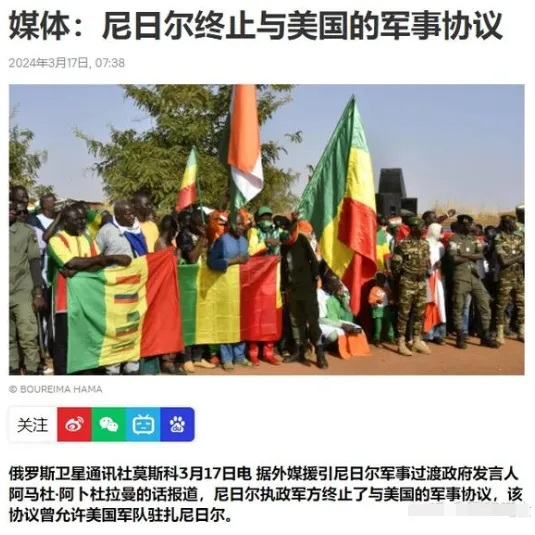
\includegraphics[width=9cm]{2024-08-08-002.jpg}
\end{figure}

美军和其他军队都不一样,没人敢动,瓦格纳也不行。

2024年4月12日,俄罗斯直接出动了正规军乘坐伊尔76降落在尼日尔,以绝对优势的兵力把美军基地给围了起来,准出不准进,断绝所有物资运输,同时让尼日尔颁布禁空令,禁止任何飞机在美军基地起降,具体禁空的武力措施由俄罗斯执行。

最后美军乖乖撤离了,军事基地直接留给了俄军。

为了解放尼日尔,俄罗斯出了大力,最终驱逐了法国和美国对尼日尔的全部驻军,收个5成收益不过分吧。

尼日尔能否也驱离俄军,彻底独立,从此自己全拿收益,谁都不分?

这个是不可能的事情,因为铀矿是特殊商品,不是你想卖就卖的,没有五常的许可你一块都别想卖,所以五常里面你至少得找一家抱大腿,得罪了法国得罪了美国,英美又是一家,中国常年不插手外国内政,如果还不想给俄罗斯分收益,那尼日尔以后就别想卖铀矿了。

然后就是制裁,尼日尔这么搞,法国和美国是不可能给好脸色看的,而尼日尔又是个内陆国,随随便便就能彻底封锁,如果没有俄罗斯撑腰来提供尼日尔所需的粮食和工业品,那尼日尔是绝对不敢和法国美国翻脸的。

\zd{法国给8\%还只能存在法国银行购买法国指定商品,俄罗斯给50\%而且任由尼日尔自由支配。}

\zd{大约直接收益翻十倍那种,所以只要俄罗斯有那个力量驱逐法军和美军,尼日尔就会毫不犹豫的投入俄罗斯的怀抱。}

而之所以定50\%的分成比例,是因为俄罗斯在其他非洲国家也是这个比例,此乃“行规”,这个比例足以让非洲国家感恩戴德的支持俄罗斯,所以就这个比例了,既然获得的支持度已经足够,那更大比例俄罗斯也是不愿意给的。

剥削度达92\%甚至更多的情况在非洲比比皆是,而最近法国被俄罗斯颠覆的控制地区也不止尼日尔一国。

2023年1月,尼日尔隔壁的国家布基纳法索发动了政变,推翻了亲法政府,新生政府要求法军离开该国。

法国被迫同意撤军,随后布基纳法索民众在街头集会庆祝,高举“打倒帝国主义”的标语。

\begin{figure}[H]
    \centering
    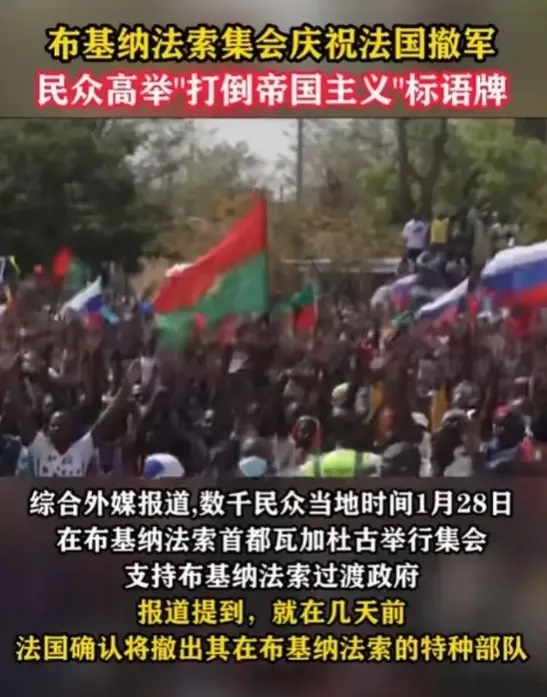
\includegraphics[width=9cm]{2024-08-08-003.jpg}
\end{figure}

\zd{这种古老的标语具备极强的历史感,如果我不说,你根本不会想到这居然是2023年的新闻。}

而法国之所以这么麻溜的撤军,是因为自2022年11月以来,布基纳法索的瓦加杜古地区就发生了一系列针对法国的示威活动,甚至有人袭击了法国大使馆和特种部队军营,还有很多民众挥舞着俄罗斯国旗,法国无力控制该地区局势。

这些非洲国家政变后敢驱离法国军队,那是因为政变是在法国军队已经控制不住该地区后才发生的,不要因果倒置。

\zd{不是说法军眼睁睁的看着当地政变,然后眼睁睁的看着自己被驱离,什么都不做就投降走人,政变是法军争夺当地控制权失败后的结果,而不是起因。}

作为“解放”布基纳法索的报酬,俄罗斯要当地金矿的5成收益,对此布基纳法索感恩戴德。

而隔壁的国家马里,也是在俄罗斯的力挺下获得了解放,法国驻军被驱逐。

\begin{figure}[H]
    \centering
    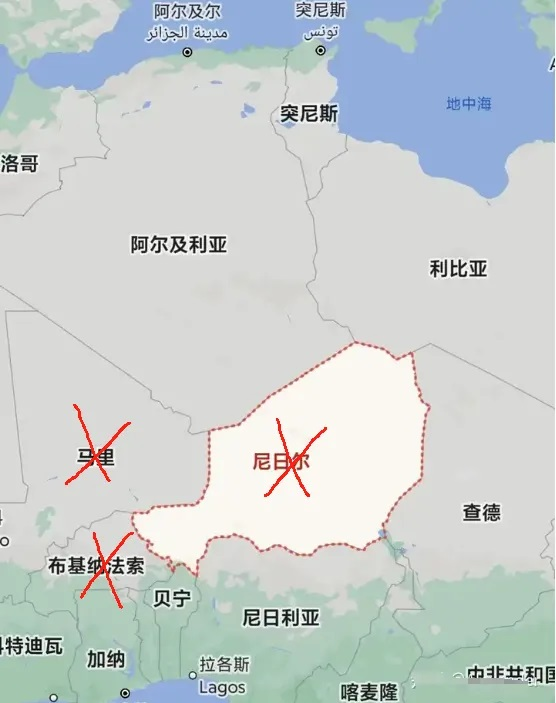
\includegraphics[width=9cm]{2024-08-08-004.jpg}
\end{figure}

更上面的国家阿尔及利亚,国歌的歌词写的就是“法国啊,你们的大势已去矣。法国啊,算账的日子已接近”,这次还在巴黎奥运会被唱响了。

\begin{figure}[H]
    \centering
    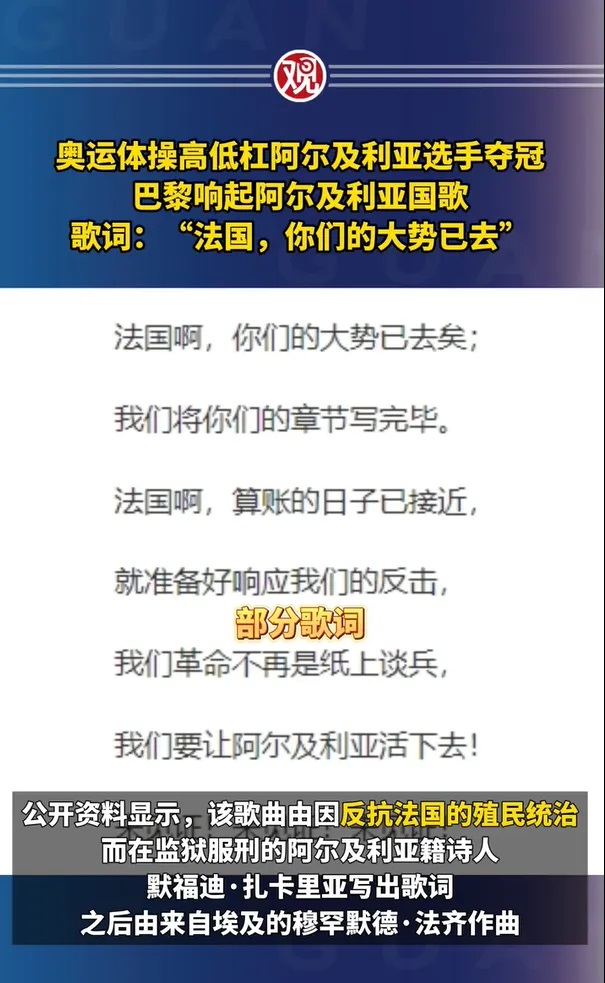
\includegraphics[width=9cm]{2024-08-08-005.jpg}
\end{figure}

阿尔及利亚当年独立了,但下面的马里、布基纳法索和尼日尔都还在被法国控制,不过这次被俄罗斯一口气全给“解放”了。

而类似的事情在非洲多个地区频繁发生着,法国雇佣军团和俄罗斯的瓦格纳在多个角落进行反复厮杀,争夺当地的控制权和经济利益。

凡是被瓦格纳控制的地区,俄罗斯的开价都是50\%,明码标价的统一规则。

\begin{figure}[H]
    \centering
    
\includegraphics[width=9cm]{2024-08-08-006.jpg}
\end{figure}

面对这一报价,那些非洲国家都感恩戴德,都视为被“解放”,因为法国、英国等的报价要黑的多。

这次被俄罗斯一口气连续拔除了三个国家的收益,虽然对法国在非洲的所有收益来说还不至于动摇根基,但也达到了非常肉痛的地步,因此法国对俄罗斯一点好脸色都没有,巴黎奥运会直接禁止俄罗斯参加。

\zd{但对俄罗斯来说,能否参加奥运会这算什么,你们都在乌克兰挑事搞我了,我肯定要在自己够得着的地方反过来搞你们。}

\zd{搞完了北非地区还要搞中非地区,只要还推得动那就一直推,以前为了维护和欧洲的关系不愿碰,现在没这个顾忌了。}

\begin{figure}[H]
    \centering
    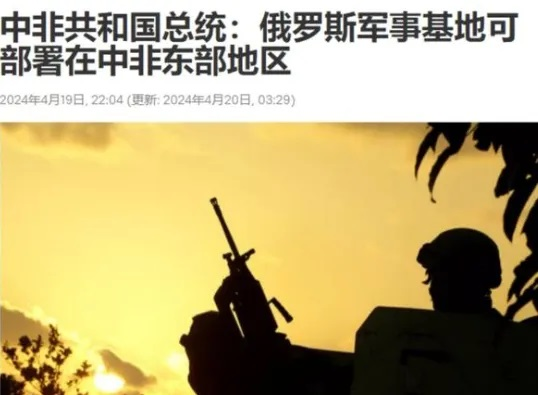
\includegraphics[width=9cm]{2024-08-08-007.jpg}
\end{figure}

如果把扣除在非洲殖民地国家获得的收益,那法国人的收入应该和意大利差不多。

没有殖民地收益,法国早就退出五常了,而英国也是类似情况。

至于美国,剥削的手段没那么直接暴力,比例也没那么高,但却可以剥削全球,所以日子过的也很好。

靠着在非洲获得的利益,英法才维持了帝国的余晖。

中国人没有殖民经验,5000多年历史中如果占据了一块新地盘,那么做的事情肯定是改土归流,固有思维就是千方百计把这块新地盘彻底消化吸收,让上面的人口认同自己是中国人。

因此中国根本无法理解为什么英国当年成为了日不落帝国,占了很多地方足足300多年,然后一夜之间就能分崩离析,而这些地方的人根本不认同自己是英国人。

对法国这种占据了尼日尔一百多年,满脑子想的就是拿走92\%的收益就够,其他不想管的行为,中国也无法理解。

同样英法以及欧美人,也无法理解为什么中国要去非洲修铁路修公路,教非洲人种水稻小麦。

\zd{这么做是图啥,欧美人非常费解,他们的历史和文化无法解释这一行为的动机。}

但实际上我们这么做,是为了百年后乃至于数百年后布局。

地球这么大,中国只占了陆地面积的7\%,当年的老祖宗根本不知道外面还有这么大的地方也就算了,如今我们知道了,那基因就被激活了。

四分五裂的地球一看就不完美,大一统才是地球的最终归宿。

欧美人认为不可能,地球永远不可能统一,再强的国家都不可能统一全球,甚至欧洲都不可能统一,必须分裂为大量的国家才能把彼此的日子过好,英美当年实力冠绝全球的时候,送上门的国家和人口都不要,因为如果要了就会引发本国内部的巨大矛盾冲突。

但我们中国人,哪怕是老百姓都不会这么认为,我们从不认为占领一个地方长达300年之后还无法融合。

\zd{占不住那是可能的,融不了那是不可能的,我们国家的历史上没有融不了这样的情况出现过。}

按中国人的思维,地球是早晚被某一个国家统一的,这是必然结局,如今四分五裂只是时机未到而已。

\zd{根据春秋战国时期的历史,争一时之长短是没有意义的,春秋战国的多个霸主最终的下场都很惨,一门心思苟起来发育,只要土地和人口其他什么都不管,不断提升国力的秦国才笑到了最后。}

到了最后那个临界点,综合国力加起来远胜秦国的六国,在积累了六世力量的秦国面前,几乎是一瞬间就被灭了。

\zd{史书记载:及至始皇,奋六世之余烈,振长策而御宇内,吞二周而亡诸侯,履至尊而制六合,执敲扑而鞭笞天下,威振四海。}

所以在奋六世之余烈之前,我们先做一点改土归流的铺垫工作,不追求一时的短期利益,更不搞剥削,这种思维非常正常。

不管是欧洲还是美国,都没有过改土归流的经验,更没有过大一统的经验,他们从不认为地球有可能统一,也不认为自己占据一个新地区之后能让上面的土著人口认同自己,比如英国就是一个活生生的例子,因此大家在都有能力拓展海外后,思路是不一样的。

欧美会认为既然这些地方不可能融合,那控制了之后当然要用最大力度剥削,现在不赶紧剥削那以后可能就剥不了了。

俄罗斯要50\%收益,居然都能被视为“解放”,得到了当地民众的高度拥护和支持。而从这个比例来看俄罗斯也没觉得自己能融合,什么长久未来也是不考虑,只是打算从英法嘴里抢点肉吃而已。

这些地方的民众慢慢等着吧,等到将来临界点到来,我们认为可以“奋六世之余烈”的时候,会让他们知道什么才是真正的解放。

\zd{因为这些国家对非洲的统治,实在是太黑了。}

\end{document}

